\section{Representación gráfica de la solución y su verificación}
\label{sec:representacion}

La solución se representa con un modelo CAD integrado en FreeCAD y con planos normalizados emitidos en SolidWorks. El modelo reúne la mesa con sus centradores, el traslado, los rieles y pedestales, el sistema de aspersión, el soporte superior, la cabina, los tanques, la bomba, el tablero y el drenaje. Los componentes comerciales se representan con los modelos de sus fabricantes cuando estuvieron disponibles. La Figura~\ref{fig:cad-maquina} muestra el conjunto.

\begin{figure}[htbp]
\centering
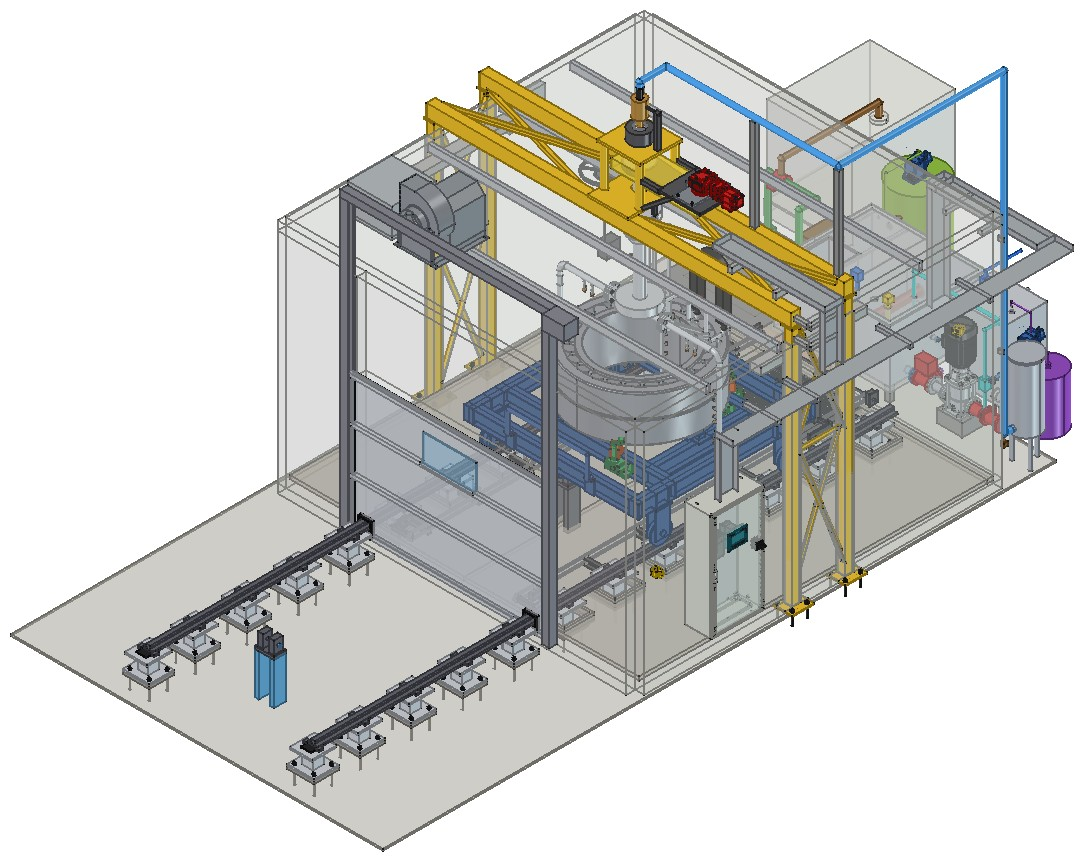
\includegraphics[width=0.70\textwidth]{cad_maquina_iso.jpg}
\caption{Modelo integrado de la máquina con la cabina transparente: mesa sobre rieles y pedestales, soporte superior con el motorreductor, distribuidor en U, tanques, bomba, tablero y puerta. Elaboración propia en FreeCAD.}
\label{fig:cad-maquina}
\end{figure}

\subsection*{Planos}

Se emitieron 34 planos con cotas, ajustes, tolerancias, lista de piezas y rótulo, más el esquema hidráulico de dos hojas (Tabla~\ref{tab:planos}). Se usó el sistema ISO con proyección en tercer diedro. Las soldaduras llevan símbolos ISO 2553 \cite{iso2553}, y las tolerancias generales son ISO 13920 clase B en los conjuntos soldados e ISO 2768-mK en las piezas mecanizadas. El Anexo~\ref{anx:planos} reúne los planos de conjunto y de los subconjuntos principales.

\begin{table}[htbp]
\centering\small\singlespacing
\caption{Planos emitidos}
\label{tab:planos}
\begin{tabularx}{\textwidth}{@{}lrY@{}}
\toprule
\textbf{Grupo} & \textbf{Cant.} & \textbf{Contenido}\\
\midrule
Mesa & 8 & Conjunto, bastidor con soldaduras, apoyo sectorial, rueda, topes (2), manillar y bloqueo central\\
Traslado y riel & 2 & Doble cadena con volante y pedestal del riel\\
Centradores & 16 & Dos de referencia y el empujador, con soporte y despiece\\
Aspersión & 6 & Sistema, eje y cubo, U, brazo, lanza y red\\
Soporte superior & 2 & Conjunto, base del poste y nudo viga--poste\\
Esquema hidráulico & 1 & Circuito y lista de componentes, en dos hojas\\
\midrule
\textbf{Total} & \textbf{35} & \\
\bottomrule
\end{tabularx}
\end{table}

\subsection*{Verificación del modelo}

Sobre el modelo final se hicieron tres revisiones independientes. La primera fue una auditoría geométrica en FreeCAD, que clasificó 146 solapes: todos son uniones representadas por solape u holguras internas ya declaradas, y ninguno es un choque nuevo. La segunda fue un barrido del traslado de 3320 mm cada 40 mm, con 292 piezas móviles frente a 323 fijas; marcó tres pares, dos del pasador de bloqueo dibujado insertado y uno de un objeto que agrupa bujes fijos y móviles, y ninguno es un choque real. La tercera fue la detección de interferencias en SolidWorks, como segunda opinión con otra herramienta. Marcó 79 interferencias en el conjunto de la mesa, 13 en el centrador empujador, 5 en el soporte de su pivote y 1 en el tope de 190$^\circ$; todas son uniones representadas por solape, ya declaradas. Los topes de 60$^\circ$ y 300$^\circ$, el traslado y el pedestal no tuvieron ninguna.

Las interferencias que quedan son representaciones del modelo y no choques, pero siguen dibujadas así. SolidWorks revisó cada ensamble por separado; las interacciones entre subsistemas las cubren la auditoría y el barrido. El barrido revisa sólidos cada 40 mm, no simula la cadena en movimiento y toma la U estacionada a 0$^\circ$. Los planos no están liberados para fabricación: faltan los planos de pieza de las barras, que hoy figuran en la lista de corte, y los de la cabina y el bloque portaboquillas. La evolución de la geometría desde la mesa circular hasta la configuración actual se registra en el Anexo~\ref{anx:iteraciones}.
